\section{Einleitung}

Dies soll eine \LaTeX{} -Vorlage für den persönlichen Gebrauch werden. Sie hat weder einen Anspruch auf Richtigkeit, noch auf Vollständigkeit. Die Quellen liegen auf Github zur allgemeinen Verwendung. Verbesserungen sind jederzeit willkommen.

\subsection{Zielsetzung}
Ziel dieser Arbeit ist es, Grundlagenwissen zu vermitteln. Ich erörtere die grundsätzlichen Unterschiede zwischen dem klassischem "Linearen" -- Fernsehen, dem Pay-TV und dem Konsum von TV -- Inhalten per Streaming.

\subsection{Aufbau der Arbeit}
Kapitel 2 enthält die Inhalte des Thesis-Days und alles, was zum inhaltlichen erstellen der Thesis relevant sein könnte. Kapitel 3 wichtige Anmerkungen zu \LaTeX{}, wobei die wirklich wichtigen Dinge im Quelltext dieses Dokumentes stehen.

\begin{figure}[H]
\begin{center}
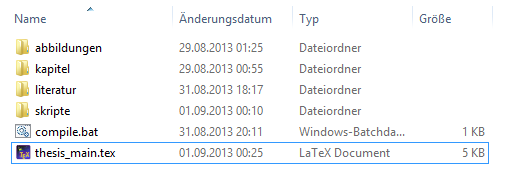
\includegraphics[width=0.9\textwidth]{verzeichnisStruktur}
\caption{Verzeichnisstruktur der \LaTeX{}-Datein}
\end{center}
\end{figure}
